\chapter{Mapping}
An active compensation system can only compensate those fields well, which its coil system can create. The question is


A mapping campaign is planned in the experimental hall, where the n2EDM experiment is going to be located. There are numerous magnetic sources in the vicinity of the site, causing the magnetic environment to be unusually complex. Taking a number of magnetic field maps will provide knowledge necessary to make sure, that the n2EDM compensation system will be able to cope with the environment. A 2.5m high mobile tower with 10 3-axis magnetic field sensors has been constructed. The position and orientation of the tower is measured with cable extension transducers, which makes the mapping process as simple as sweeping an area with the tower. Reproducibility of the maps measured with the device was proven to be better than \SI{0.5}{\micro\tesla}.

\note{maybe cite also:~\cite{Bodmer2013}}



\section{The idea}
An essential input to designing the n2EDM active magnetic field compensation system was the scope of fields that would need to be compensated. There were numerous magnetic sources in the vicinity of the \note{mention the size of the hall} site, many of them dynamic, causing the magnetic environment to be unusually complex. Taking a number of maps of the magnetic field was planned to collect the information.

Speed was valued more than precision. The shorter it would take to map the field in the whole area, the less it would be influenced by varying external conditions. Also, the dynamics of the magnetic environment favoured taking multiple maps under different conditions, rather than few precise ones.
The implemented solution was a mobile tower equipped with magnetic field sensors at different heights, whose position and orientation could be measured while it was sweeping the area being mapped.

\begin{figure}
  \centering
  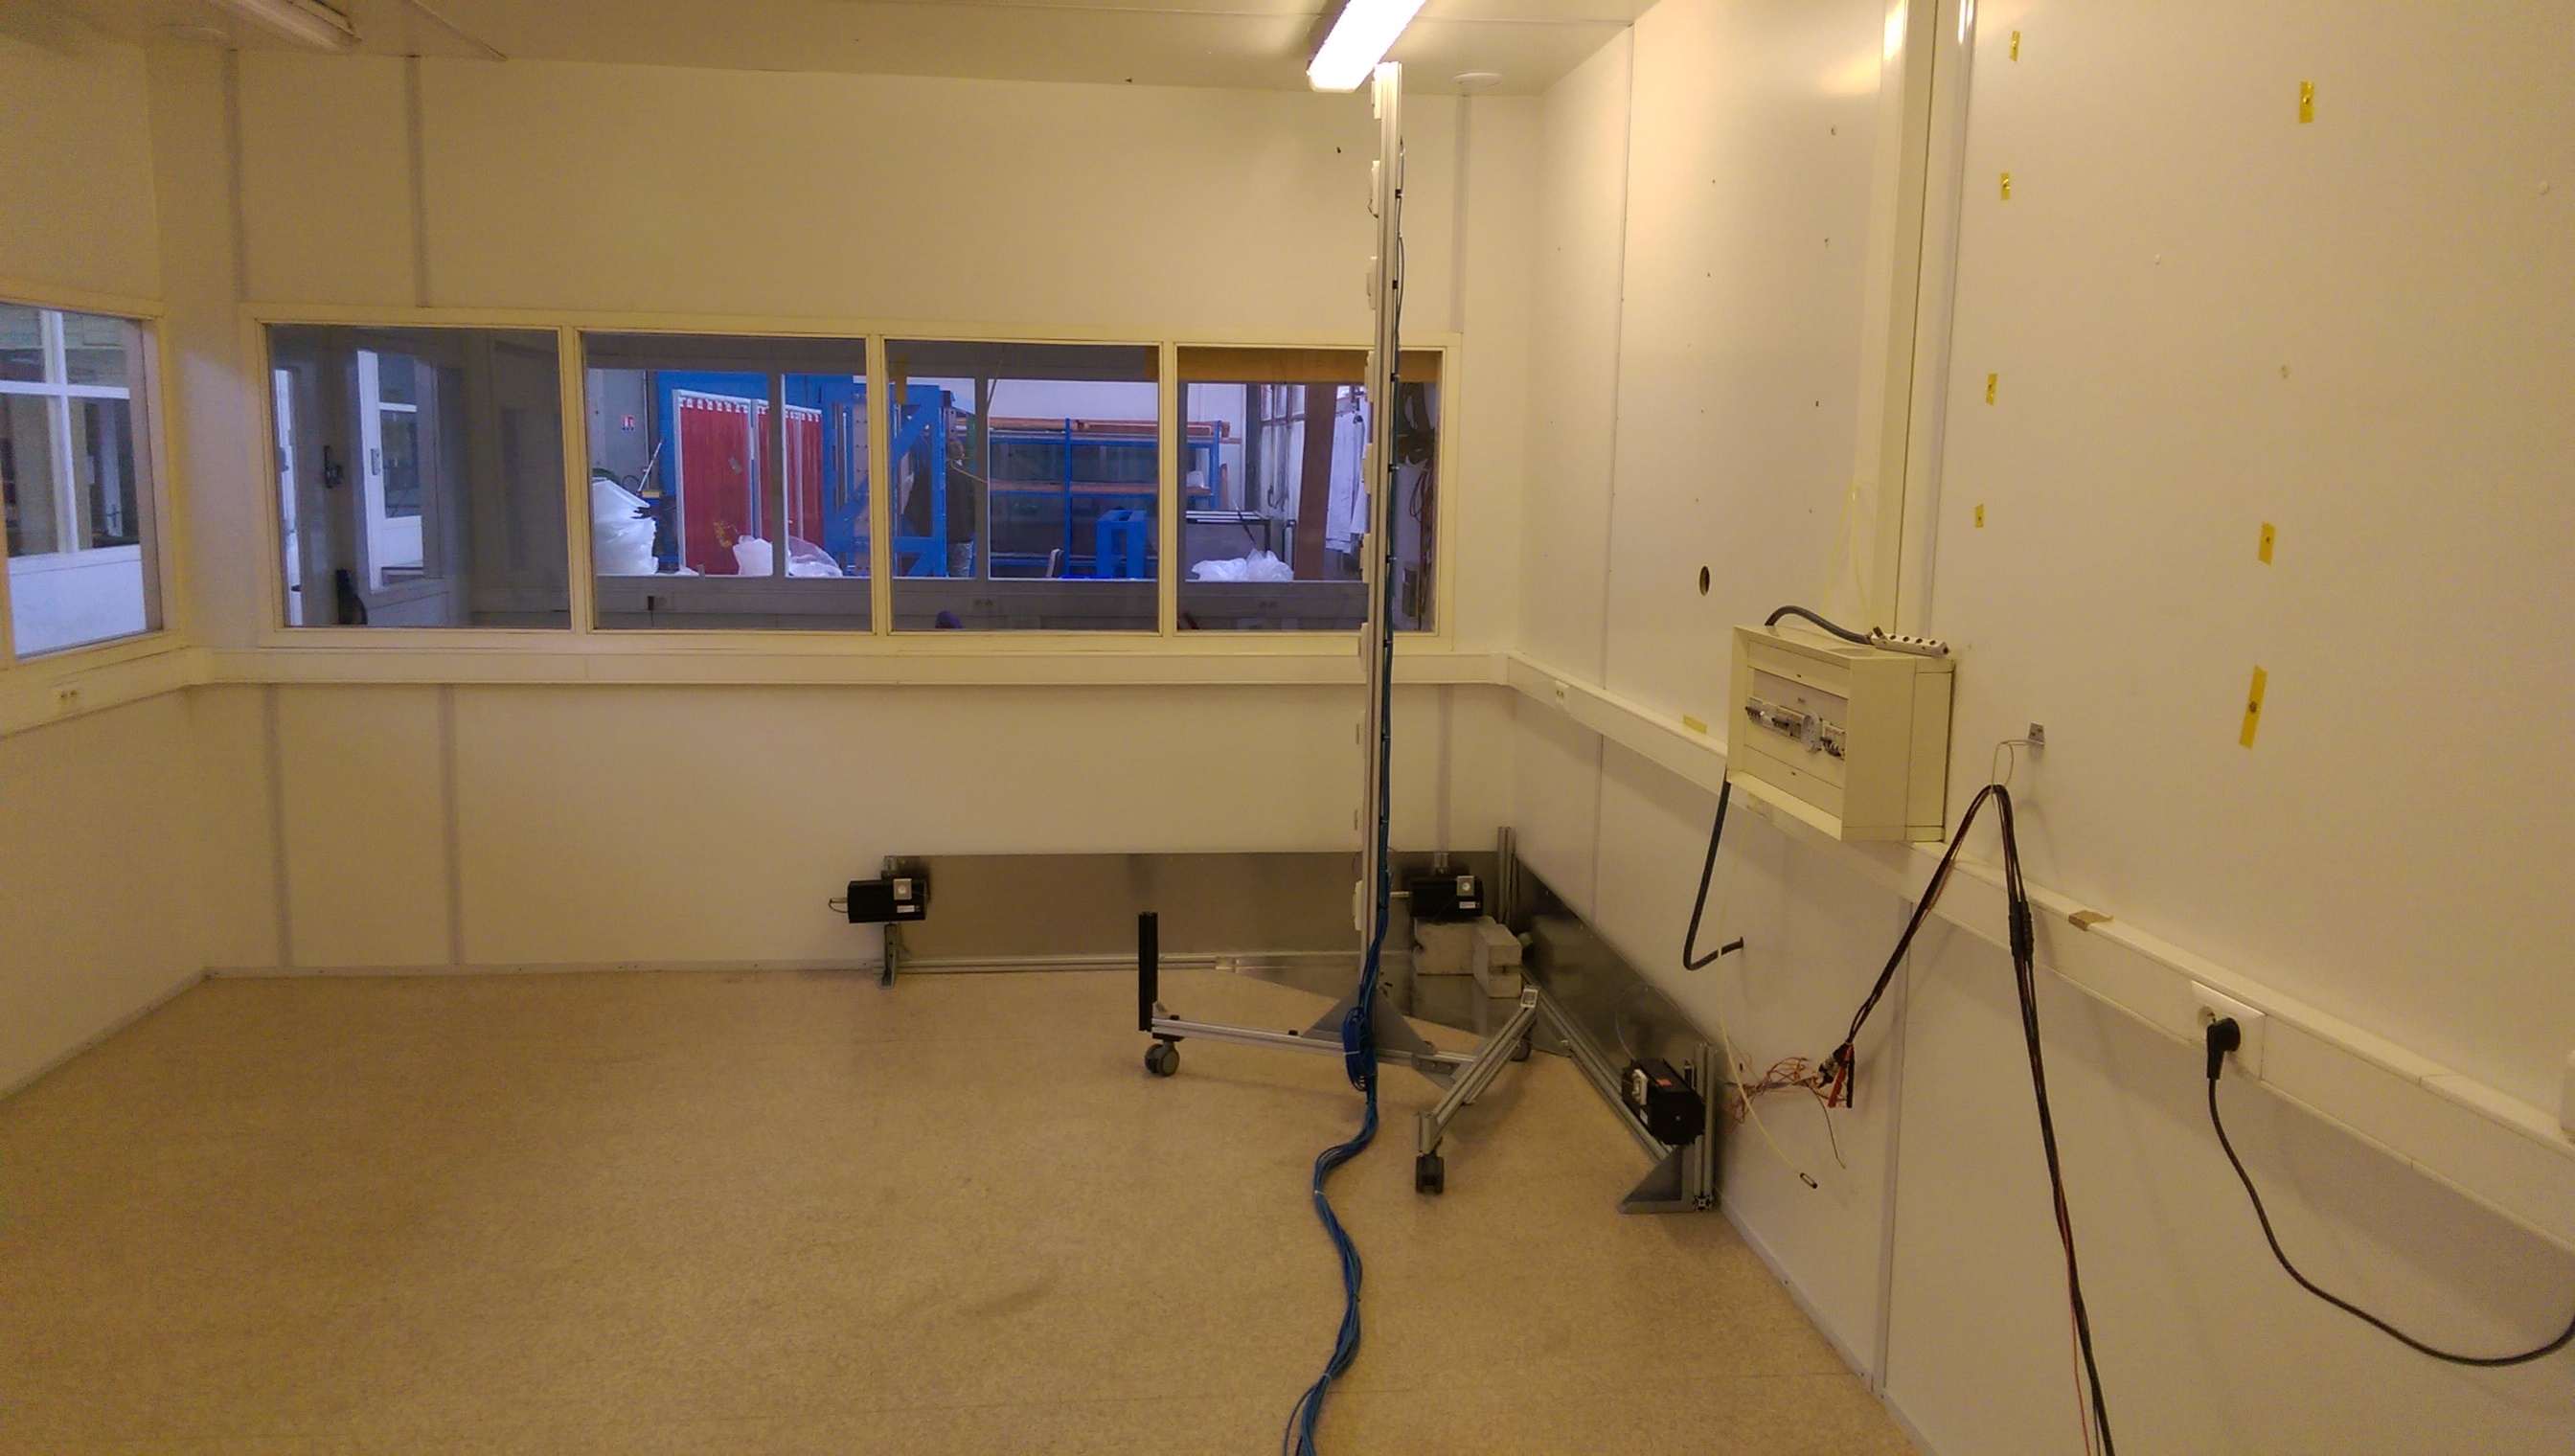
\includegraphics[width=\linewidth]{gfx/mapping/lpsc/setup.jpg}
  \caption{The small-scale prototype of the magnetic field mapper. The mobile tower has ten fluxgate magnetometers attached to it. A bundle of readout cables is visible coming out of the tower. Behind, a rigid L-piece is visible with three string potentiometers mounted on it. A string is extended from each to the tower. \note{crop the picture still}}\label{fig:mapping_bastille_setup}
\end{figure}

% present tense - describing a picture
\marginpar{For maximal linearity string potentiometers are constructed in a way, that the wire is wound flat in one layer only.}
A small-scale prototype setup is pictured in Fig.\,\ref{fig:mapping_bastille_setup}. The tower is \SI{250}{\centi\metre} high and has ten fluxgate magnetometers mounted on it. Behind the tower, in the corner, a rigid L-piece is visible. 
\marginpar{Other names for a string potentiometers include: cable-extension transducer, draw-wire sensor and string pot.}
It is carrying three black elements, string potentiometers, each with a thin wire coming out of it, the other end attached to the tower. Inside a string potentiometer the wire is wound on a spring-loaded spool, the spool attached to a potentiometer.
The potentiometer gives an analogue signal proportional to the extension of the wire. The combined information from the three sensors was used to determine the position and orientation of the tower.



\section{Principle of a string-potentiometer--based mapper}
For a known extension of a wire the set of points where the other end can be is a circle. The position and orientation determination is, in fact, finding the intersections of those circles.
\marginpar{Other position determination methods include triangulation (measurement of angles between lines connecting a set of fixed points) and multilateration (measurement of the differences of distances between a set of fixed points).}
In general, the problem of determining the location based on the measurement of the distance to a set of fixed points is called \emph{trilateration}.

\begin{figure}
  \centering
  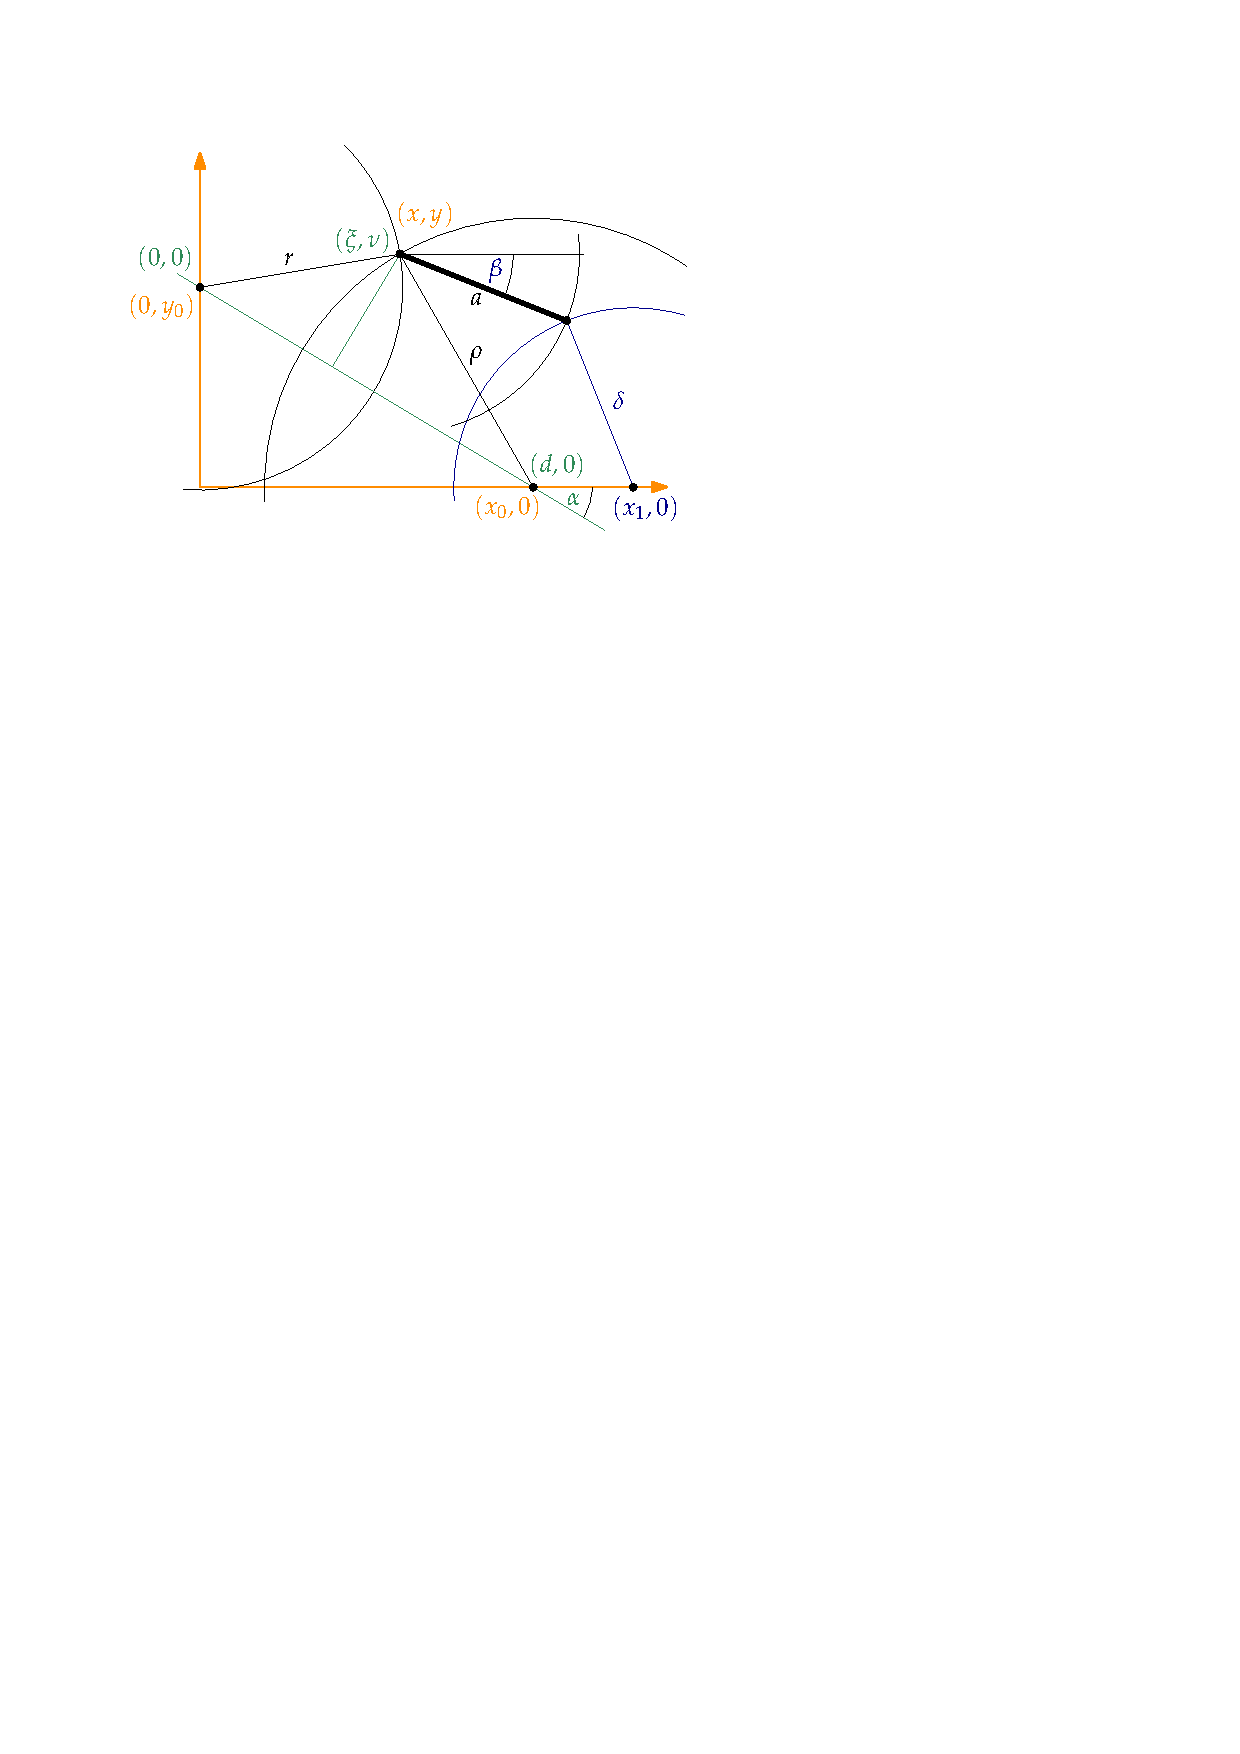
\includegraphics[width=0.8\linewidth]{gfx/mapping/geometry.pdf}
  \caption{The geometry of the mapper's position and orientation determination. In the orange coordinate system, the one of the `L-piece', the position of the centre of the tower, depicted as a thick black line, is $(x,y)$. The positions of the string-potentiometers used to determine the tower's position are $(0, y_0)$ and $(x_0, 0)$ and the extensions of their wires: $r$ and $\rho$. Another, green, coordinate system is depicted, in which the position of one of the string-potentiometers is $(0,0)$ and the other $(d, 0)$. The position of the tower in this coordinate system is $(\xi, \nu)$. There is also a third string-potentiometer, its string, length $\delta$, attached to the tower on an arm of a length $a$.}\label{fig:mapping_geometry}
\end{figure}

The geometry set by the circles is illustrated in Fig.\,\ref{fig:mapping_geometry}. The two string potentiometers used to determine the position are located is points $(x, y) = (0, y_0)$ and $(x_0, 0)$ (in the L-piece coordinate system, orange in the figure).
The wires of those two, their lengths $r$ and $\rho$, are connected to a single point $(x,y)$, lying directly on the vertical beam holding the sensors. We will refer to the point as the centre, even though it is not necessarily the geometric centre of the tower. The centre lies on the intersection of the corresponding circles.
For the sake of simplicity, we first give the solution for the centre's position in the coordinate system depicted in green,
% \note{maybe use the A B and C names here already}
where the first string potentiometer is in $(0,0)$, the second in $(d, 0)$, with
\begin{equation}
  d = \sqrt{x_0^2 + y_0^2} \ ,
\end{equation}
and the tower's centre is in $(\xi, \nu)$. Then: 
\begin{align}
  \xi & = \frac{1}{2d} \left( d^2 - \rho^2 + r^2 \right) \\
  \nu & = \pm\ \frac{1}{2d} \sqrt{ (-d + \rho - r) (-d - \rho + r) (-d + \rho + r) (d + \rho + r) } \ .
\end{align}
There are two solutions, symmetric around the line connecting the centres of the circles. Typically, though, it can be assumed that the tower never crosses the line.
The transformation of the solution to the `L-piece', orange, coordinate system is rotation by the angle 
\begin{equation}
  \alpha = \mathrm{ctan}\, \frac{y_0}{x_0} \ ,
\end{equation}
followed by a translation:
\begin{equation}
  \begin{pmatrix}
    x \\
    y
  \end{pmatrix}
  =
  \begin{pmatrix}
    \cos \alpha & -\sin \alpha \\
    \sin \alpha & \cos \alpha
  \end{pmatrix}
  \begin{pmatrix}
    \xi \\
    \nu
  \end{pmatrix}
  +
  \begin{pmatrix}
    0 \\
    y_0
  \end{pmatrix} \ .
\end{equation}
The orientation is determined with a used of the third potentiometer, its string attached to the tower at a distance $a$ from its centre. Then, the position of the attachment point lies on the intersection of the circle centred at $(x,y)$, radius $a$, and one centred at the potentiometer, radius equal to the measured extension of the wire $\delta$. In this case there are also two solutions, but ambiguity could be avoided by keeping the orientation of the tower approximately constant.

% in the same way, but with one circle centred in $(x,y)$, and the other at the 

% The problem of determining the orientation of the tower is, in fact, the same as the one of the position. The third string potentiometer, with the string attached to \note{there are two $d$s in the picture!} an arm of the tower (depicted in violet in Fig.\,\ref{fig:mapping_geometry}) of the length $a$. The end of the arm lies on the intersection of two circles: the one centred in the centre of the tower and radius $a$, and the one centred at the sensor end of the third potentiometer with the length equal to the wire extension.

\note{Comment on the sensitivity here. The solution is best conditioned, when the angle of the intersection of the circles is large. There is a problem, in particular, in the ``upper-left corner''.}



\section{LPSC campaign}
The mapper setup was used to perform a mapping of the magnetic field in Laboratoire de Physique Subatomique \& Cosmologie (LPSC) in Grenoble, France in the days 6.-10.03.2017, with the much appreciated help of Rémi Faure, Guillaume Pignol and Dominique Rebreyend. The goal was to map two rooms, referred to as \emph{Bastille} and \emph{Chalet}. The rooms were considered to host a magnetic-field sensitive setup for ${}^{199}$Hg magnetometry. In particular, gradients above roughly \SI[per-mode=symbol]{10}{\nano\tesla\per\centi\meter} cause an increase in the depolarisation rate of the mercury atoms.

A photograph of the mapping setup is shown in Fig.\,\ref{fig:mapping_bastille_setup}. The movable \SI{2.5}{\meter} high tower was equipped with ten 3-axis fluxgate magnetic field sensors. The stationary coordinate system featured three string potentiometers spanned to the tower. The string pots were equipped with a custom made attachments that allowed the string to come at an angle out of the device. Two of the strings were attached to a point where the vertical beam with the fluxgates is, the third (left on the picture) was attached to the black, short vertical profile on the tower.

\marginpar{Technical details of the setup: fluxgates: Stefan-Mayer FLC3--70, ADC: aoethu, string potentiometers: Micro-Eplison WDS-15000-P115-SA-P, readout frequency: xxx}

\begin{figure}
  \centering
  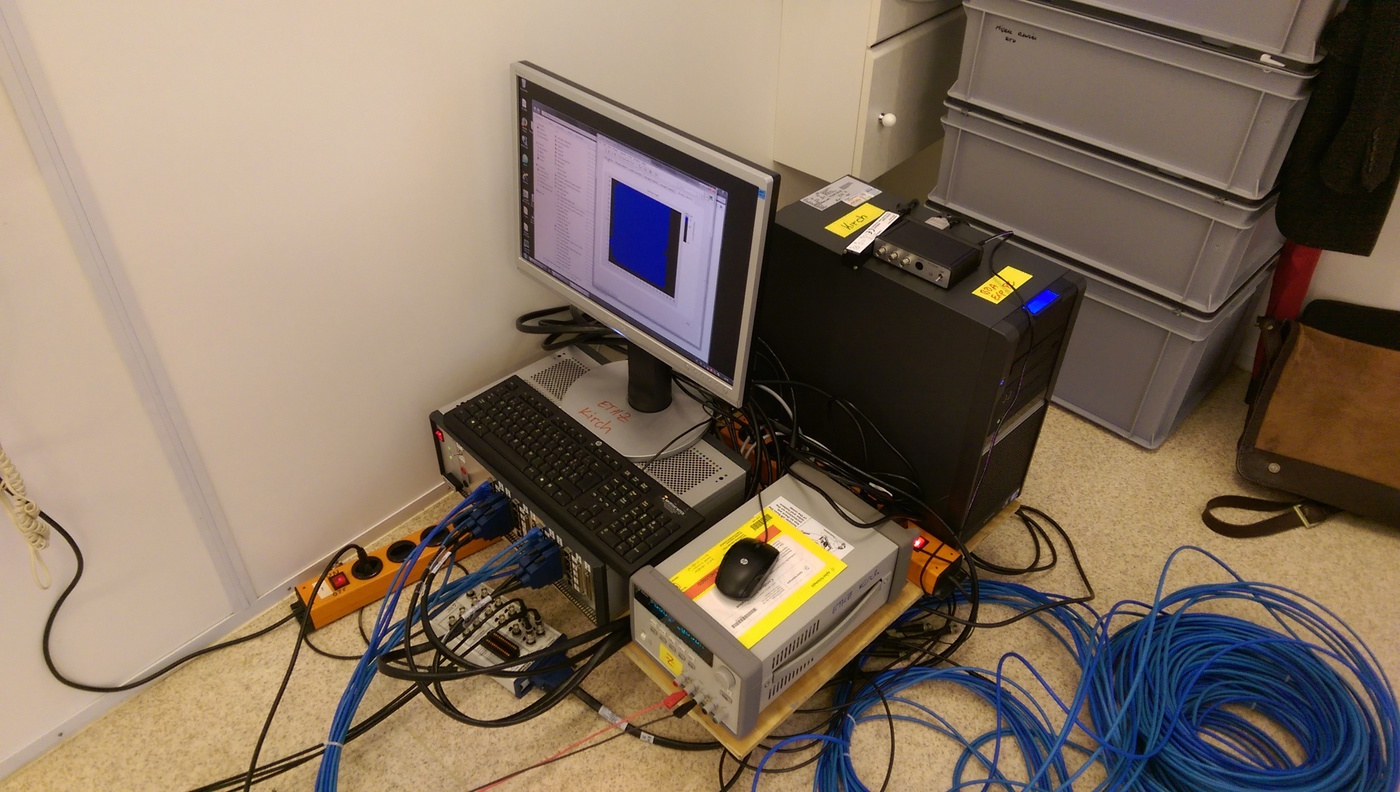
\includegraphics[width=0.9\linewidth]{gfx/mapping/lpsc/daq.jpeg}
  \caption{\ldots}\label{fig:mapping_bastille_daq}
\end{figure}

The data acquisition system, pictured in Fig.\,\ref{fig:mapping_bastille_daq}, was located on a cart. It consisted of a power supply used to put a constant voltage on the string potentiometers, a custom-built crate for the fluxgates, which supplied them with power and conditioned the incoming signals, and a National Instruments PXI crate, which simultaneously digitised the analogue voltage signals from the fluxgates and the string-pots.

\begin{figure}
  \centering
  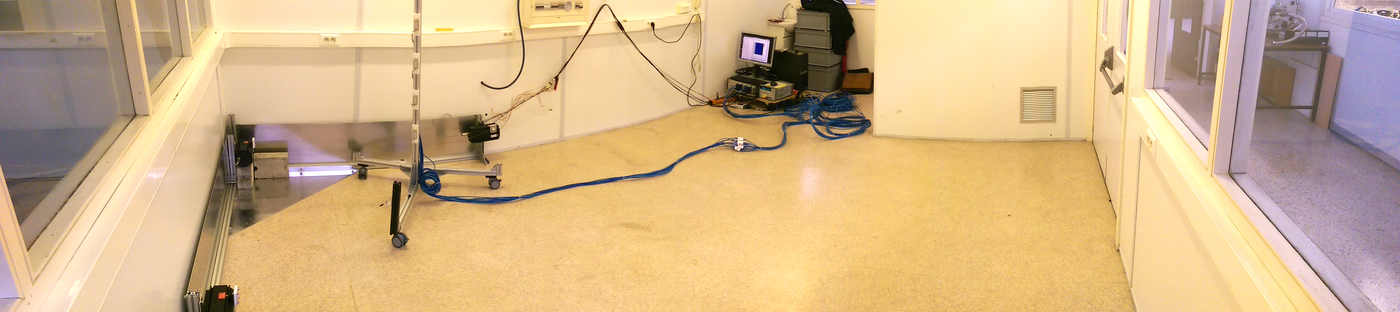
\includegraphics[width=\linewidth]{gfx/mapping/lpsc/bastille_panorama.jpeg}
  \caption{\ldots}\label{fig:mapping_bastille_panorama}
\end{figure}

A panoramic shot of the Bastille room is presented in Fig.\,\ref{fig:mapping_bastille_panorama}. The coordinate system is visible in the upper-left corner. To the right are the entrance door, in the middle a power outlet box is visible.
% Behind the wall with the power outlet box there is a pump, which has been at some point removed.
The room is a wooden structure built in a hall. made of steel beams and sheets. The room's wall with the power outlet is located close, less than 1 metre, to the steel wall of the hall. The hall features a gantry crane, several metres above the roof of the room. On the roof of the room there are air conditioning devices, standing about a metre above the roof on steel legs. The legs have rather large feet, possibly with a steel plate inside.

\begin{figure}
  \centering
  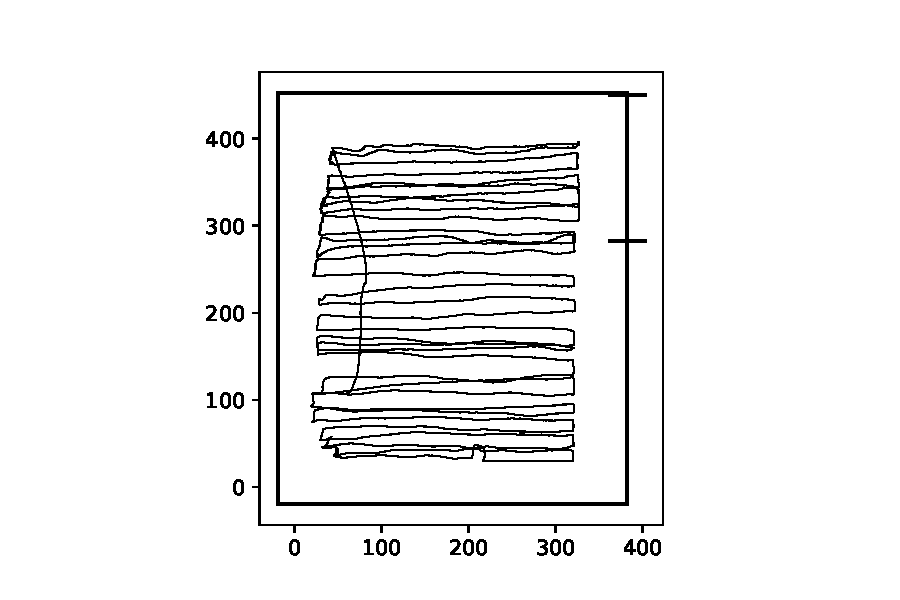
\includegraphics[width=0.9\linewidth]{gfx/mapping/lpsc/bastille_crane_away_rep_track.pdf}
  \caption{\ldots}\label{fig:mapping_bastille_track}
\end{figure}

\begin{figure}
  \centering
  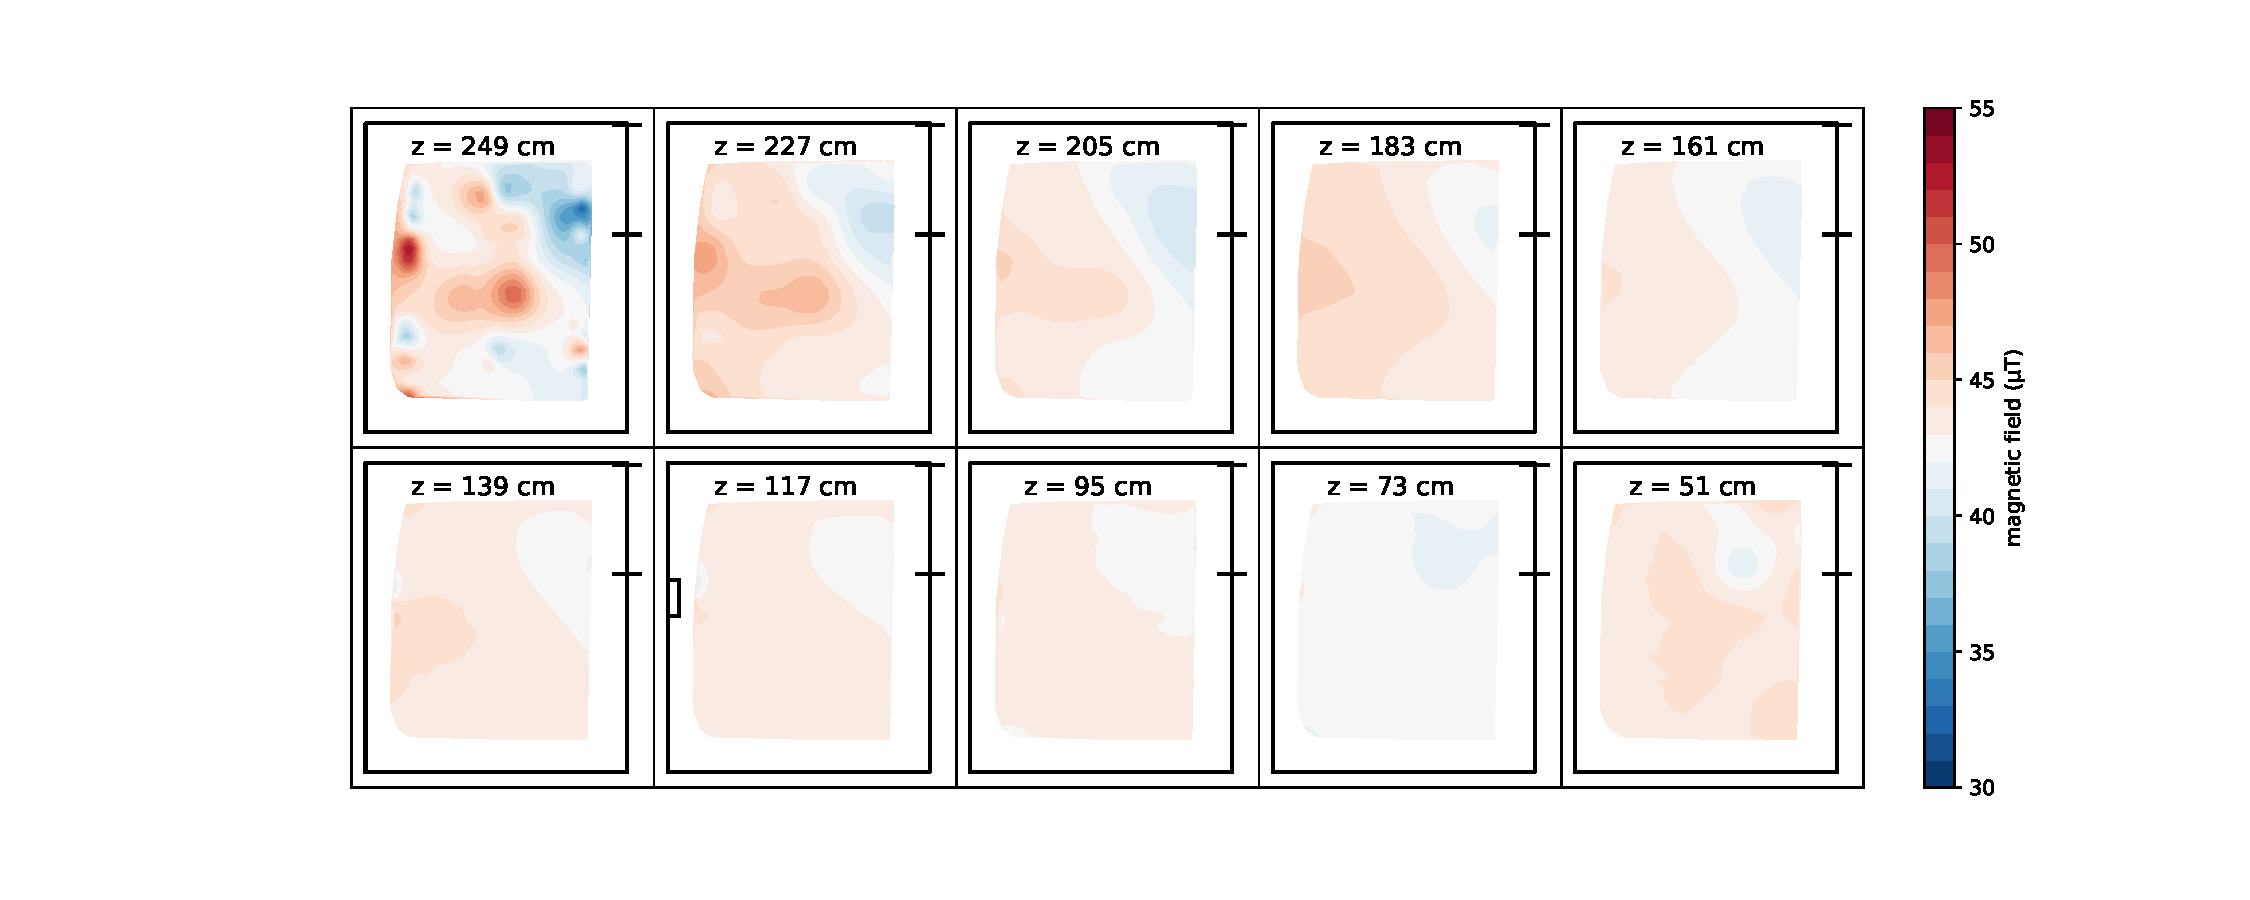
\includegraphics[width=\linewidth]{gfx/mapping/lpsc/bastille_crane_away_rep_magnitude.pdf}
  \caption{\ldots}\label{fig:mapping_bastille_magnitude}
\end{figure}

To collect a map, the tower was moved around the room by hand. Care is taken to scan the whole room and to maintain approximately the same orientation of the tower throughout the measurement. The track of one of the collected maps is depicted in Fig\,\ref{fig:mapping_bastille_track}, together with an overview of the room. \note{maybe mention, that the position was calculated on-line, too} Part of the data analysis is performed on-line. In particular the voltage readout of the string pots is translated into their lengths which are used to determine the position and orientation of the tower. This is to provide feedback during the measurements, necessary to make sure that the whole room was scanned. The resulting map was a set of points, collected at \note{give the sampling frequency}, with the position of the tower and magnetic field readout for each fluxgates. Those data are directly plotted in Fig.\,\ref{fig:mapping_bastille_magnitude}. Horizontal slices (each a different sensor) of the magnitude of the magnetic field are shown, with the height of the slice above the floor indicated. It is clearly visible, that there are localised sources of magnetic disturbance above the roof, later attributed to elements of the air-conditioning system mounted on the roof of the hut.

\begin{figure}
  \centering
  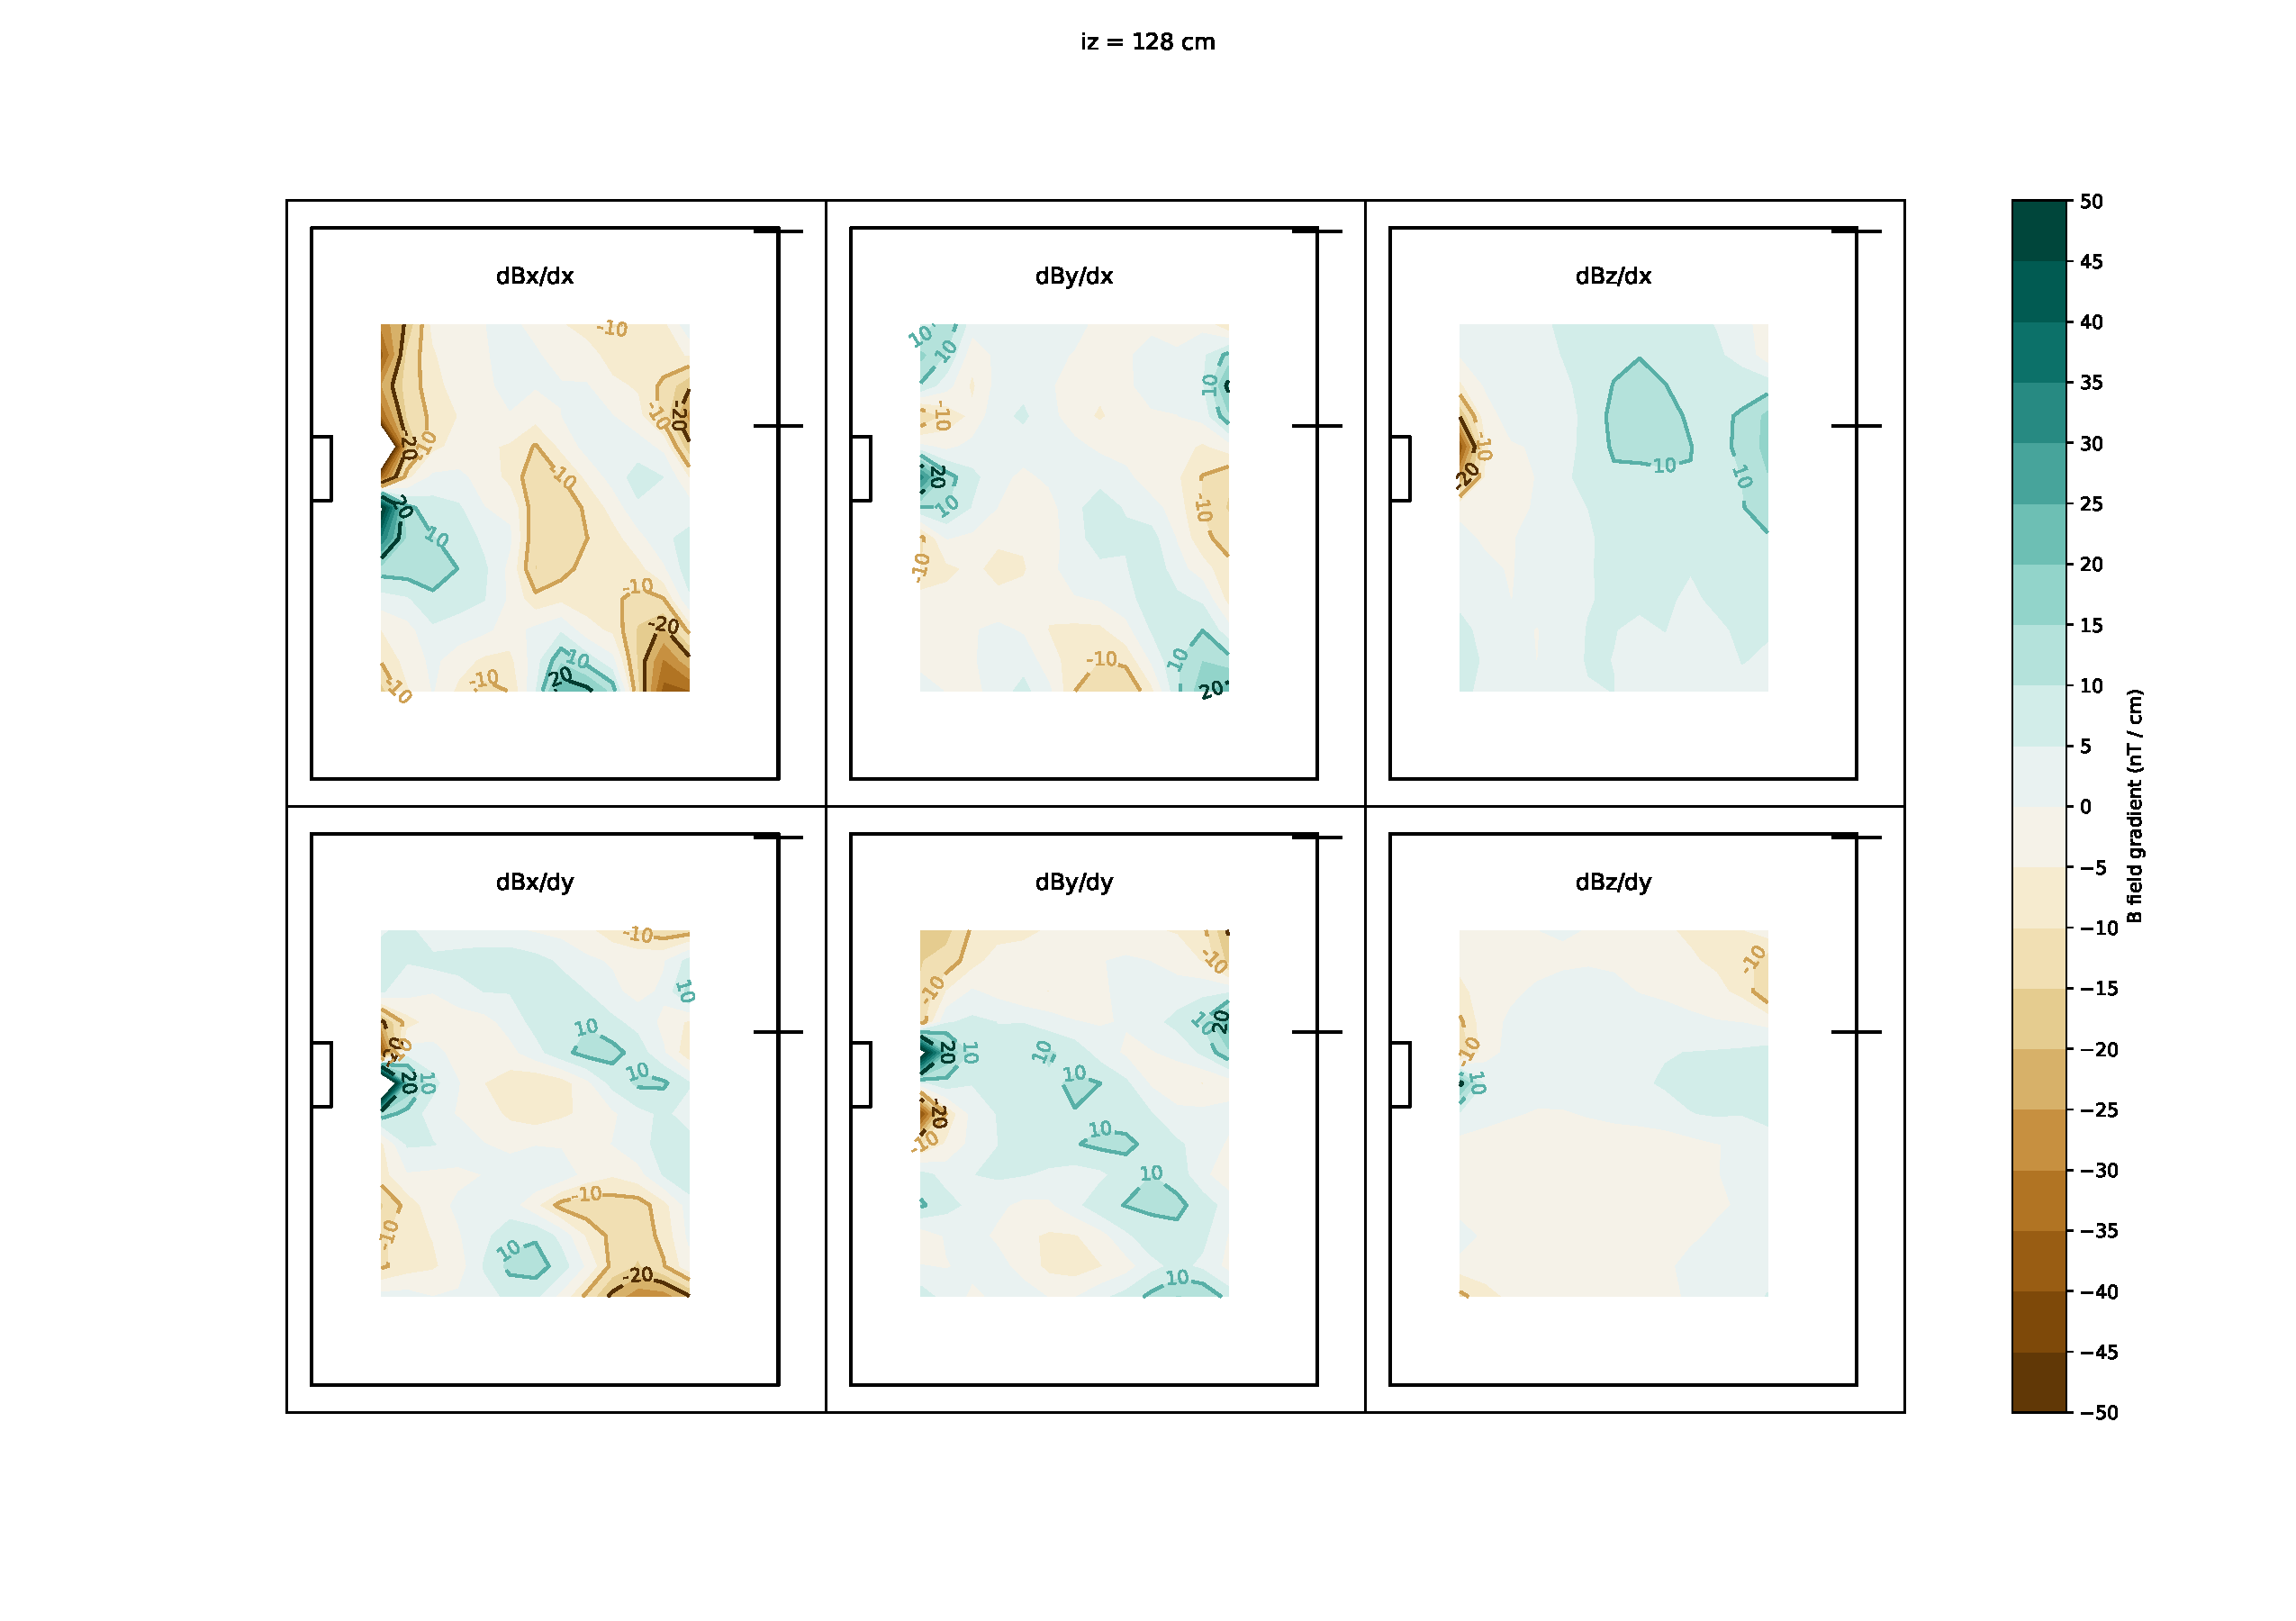
\includegraphics[width=\linewidth]{gfx/mapping/lpsc/bastille_crane_away_rep_gradient_139cm.pdf}
  \caption{\ldots}\label{fig:mapping_bastille_gradient}
\end{figure}

The mapper collects not only the magnitude of the field, but the full vector information. This can be used to produce maps of the gradient of the magnetic field. For this purpose the area is divided into pixels, and the average magnetic field is calculated in each.
The the differences between the magnetic field components in the neighbouring pixels are taken, which, divided by the separation between the pixels, are the estimates of the gradient.
For example, the dBx/dx gradient is estimated by the\ldots The map of the gradient \SI{128}{\centi\meter} above the floor is shown in Fig.\,\ref{fig:mapping_bastille_gradient}. Comment on the structures from the roof? On the left side, next to the power outlet box, large gradients above \SI[per-mode=symbol]{20}{\pico\tesla\per\centi\meter} are visible. Only ``horizontal'' gradients were estimated.
To estimate the vertical ones would require to compare the readouts of different sensors. The sensors are specified to be only $\pm 1\% \pm \SI{0.5}{\micro\tesla}$ accurate, which in a \SI{50}{\micro\tesla} field adds up to \SI{1}{\micro\tesla}. With a \SI{22}{\centi\meter} separation between the sensors, the systematic effect on the gradient would be \SI[per-mode=symbol]{45}{\nano\tesla\per\centi\meter}.

\begin{figure}
  \centering
  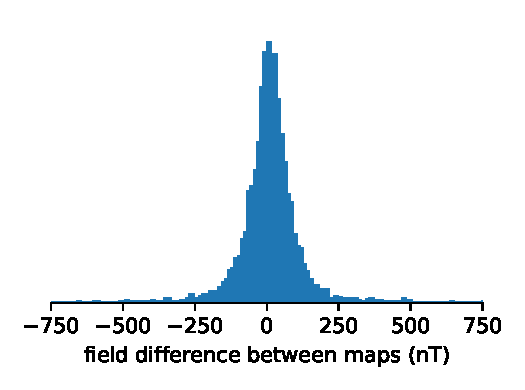
\includegraphics[width=0.8\linewidth]{gfx/mapping/lpsc/reproducibility_field.pdf}
  \caption{\ldots}\label{fig:mapping_bastille_reproducibility}
\end{figure}

Binned data allow also for direct comparison between maps. In order to estimate the reproducibility of the mapping process two maps were taken directly one after another. The maps were then, after binning, subtracted from one another. The histogram of the differences is shown in Fig.\,\ref{fig:mapping_bastille_reproducibility} (one entry is one difference in one of the components). The standard deviation of the distribution, a measure of the reproducibility, is \SI{0.14}{\micro\tesla}. The reproducibility of the gradient was estimated in the same way, yielding the standard deviation of \SI[per-mode=symbol]{3.8}{\nano\tesla\per\centi\meter}. This is better than a na\"{\i}ve estimate, which assumes that the value of the component of the field measured in one bin has a \SI{0.14}{\micro\tesla} uncorrelated error bar associated with it:
\begin{equation}
  \frac{\SI{140}{\nano\tesla} \, \sqrt{2}}{\SI{25}{\centi\meter}} = \SI[per-mode=symbol]{8}{\nano\tesla\per\centi\meter} \ .
\end{equation}
The reason is, that the for the absolute field estimate to be reproducible the system needs to be stable on a large scale -- from one map to another. For the gradient of the field to be reproducible, the system needs to be stable only from one bin to the next.

\begin{figure}
  \centering
  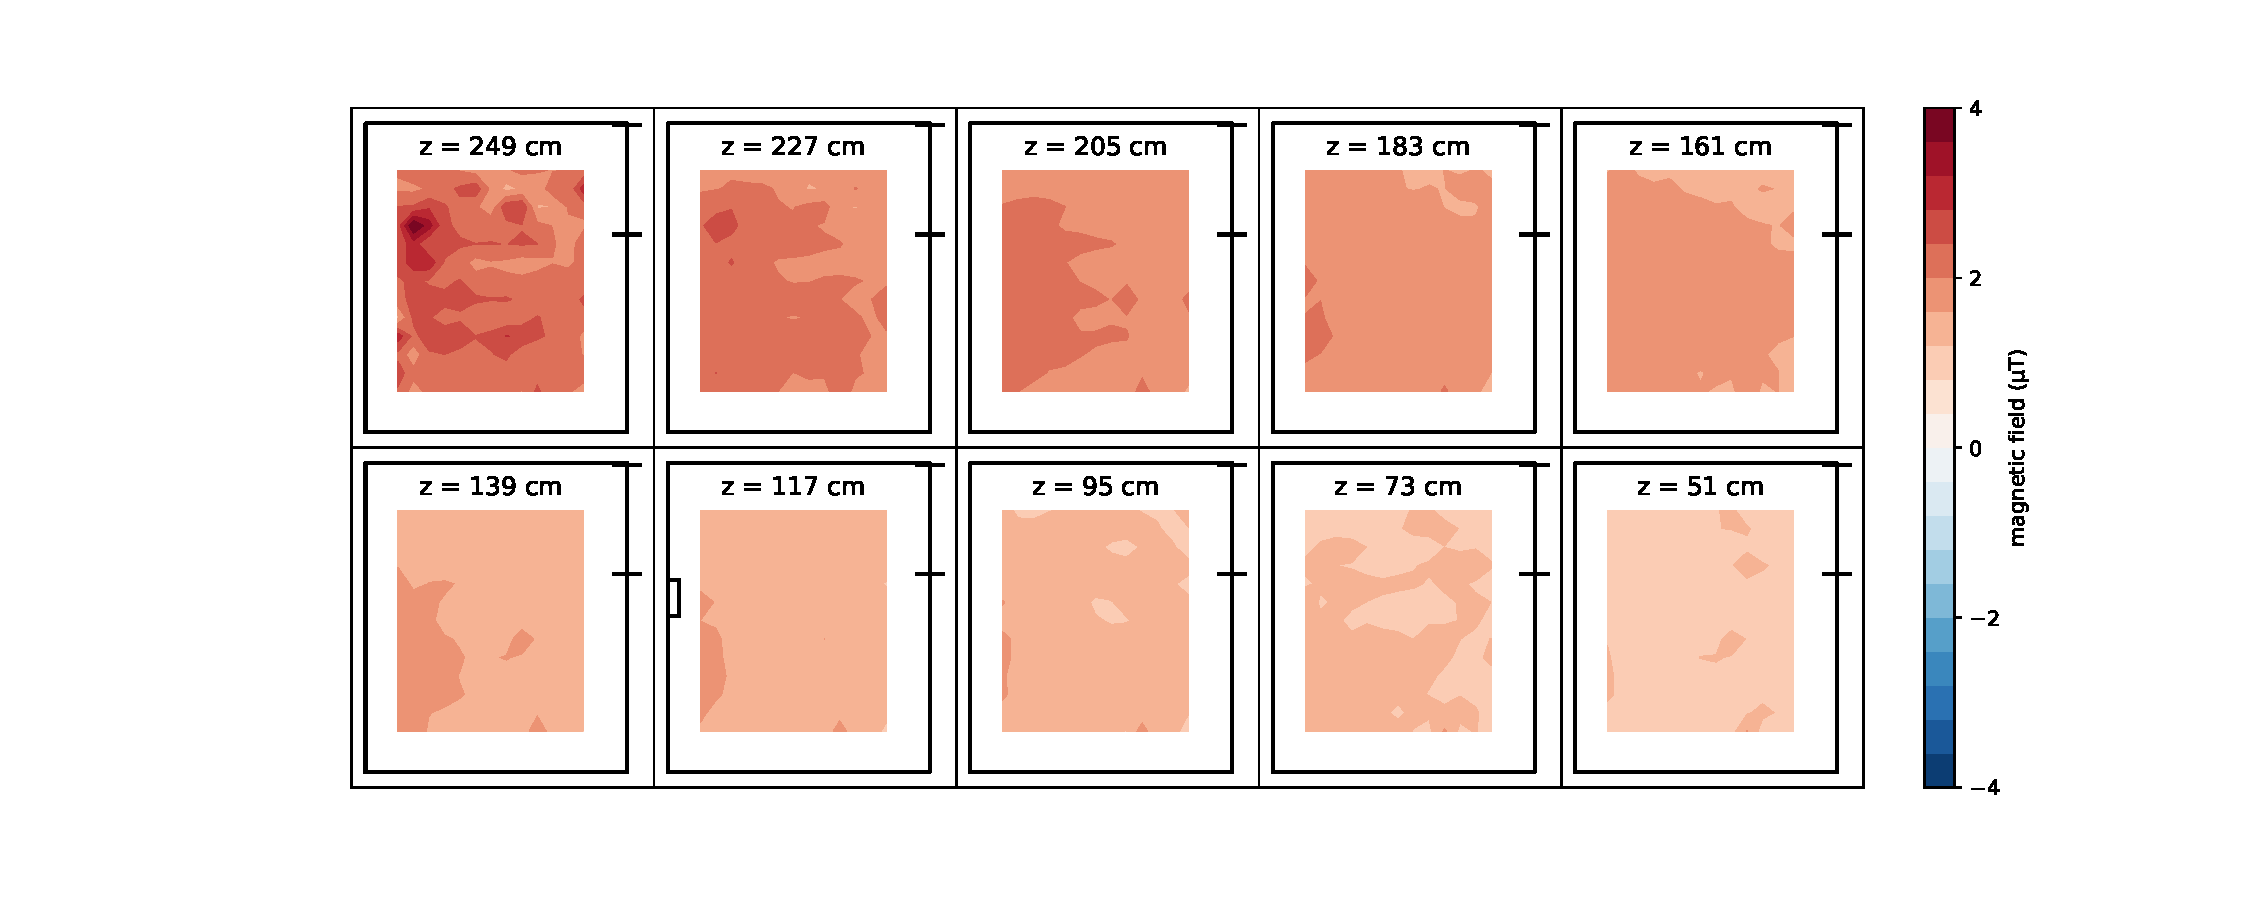
\includegraphics[width=\linewidth]{gfx/mapping/lpsc/bastille_crane_change_magnitude.pdf}
  \caption{\ldots}
  \label{fig:mapping_bastille_crane_change}
\end{figure}

Also two maps taken in different conditions can be compared. Near the roof of the hall there was a large gantry crane. In order to map the change of the field it inflicts two maps were taken: one with the crane in the far end of the hall and another with the crane directly above the hut. The maps were binned and their difference, plotted in Fig.\,\ref{fig:mapping_bastille_crane_change}, is an estimate of the field of the crane. The magnetic field produced by the crane in the hut is about \SI{1}{\micro\tesla} strong half a metre above the floor, furthest from the crane, and rises to \SI{3}{\micro\tesla} at the hut's roof. Horizontally the change is homogeneous on a \ldots level.
\mnote{A more detailed analysis of this map, maybe? But not really necessary.}


% \begin{figure}
%   \centering
%   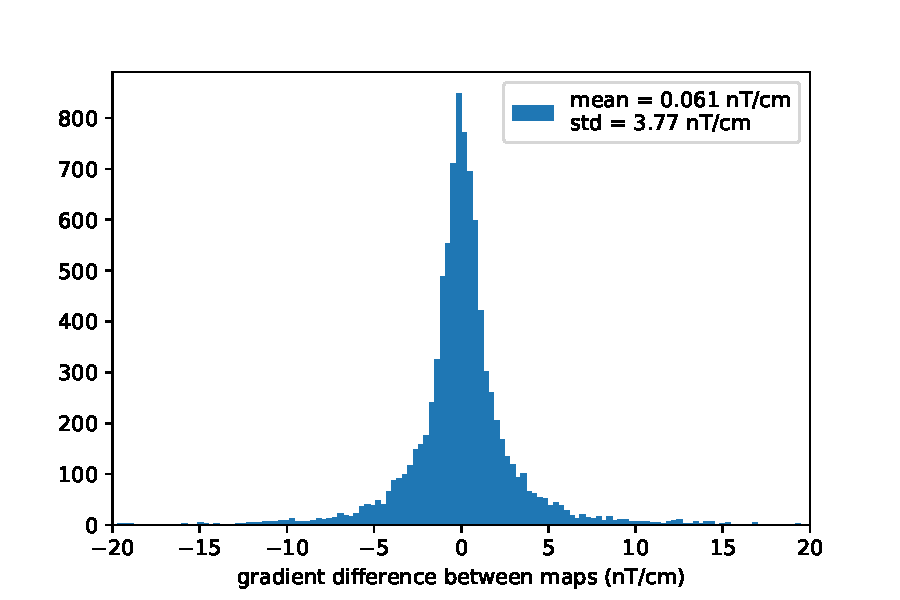
\includegraphics[width=0.8\linewidth]{gfx/mapping/lpsc/reproducibility_gradient.pdf}
%   \caption{\ldots}
%   \label{fig:mapping_bastille_magnitude}
% \end{figure}




\section{PSI Area South campaign}
\marginpar{The mapping took place in the days 18--22.12.2017 and 2--12.01.2017.}

Acknowledge that it is a joint work with Solange Emmenegger.

Describe the changes to the setup: now the geometry is like this and this. Need probably a detailed picture of the geometry of the setup and the mapper.

About the method to fit the calibration parameters to the fixed points.